

\tikzset{every picture/.style={line width=0.75pt}} %set default line width to 0.75pt        

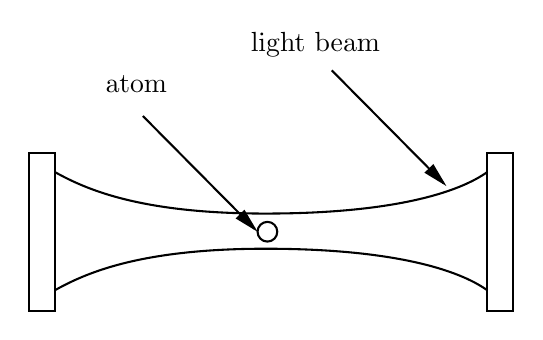
\begin{tikzpicture}[x=0.75pt,y=0.75pt,yscale=-1,xscale=1]
%uncomment if require: \path (0,300); %set diagram left start at 0, and has height of 300

%Shape: Rectangle [id:dp6401935998288966] 
\draw   (100,115) -- (87.5,115) -- (87.5,191.06) -- (100,191.06) -- cycle ;
%Shape: Rectangle [id:dp8861328448036845] 
\draw   (321,115) -- (308.5,115) -- (308.5,191.06) -- (321,191.06) -- cycle ;
%Curve Lines [id:da7513389130911845] 
\draw    (100,124) .. controls (114.5,132.06) and (140.5,144.06) .. (201.5,144.06) .. controls (262.5,144.06) and (294.5,134.06) .. (308.5,124) ;
%Curve Lines [id:da18714732754068852] 
\draw    (100,181.06) .. controls (114.5,173) and (140.5,161) .. (201.5,161) .. controls (262.5,161) and (294.5,171) .. (308.5,181.06) ;
%Shape: Circle [id:dp26153395911676935] 
\draw   (197.75,152.81) .. controls (197.75,150.19) and (199.88,148.06) .. (202.5,148.06) .. controls (205.12,148.06) and (207.25,150.19) .. (207.25,152.81) .. controls (207.25,155.44) and (205.12,157.56) .. (202.5,157.56) .. controls (199.88,157.56) and (197.75,155.44) .. (197.75,152.81) -- cycle ;
%Straight Lines [id:da08522771807029916] 
\draw    (142.5,97.06) -- (196.34,151.39) ;
\draw [shift={(197.75,152.81)}, rotate = 225.26] [fill={rgb, 255:red, 0; green, 0; blue, 0 }  ][line width=0.08]  [draw opacity=0] (12,-3) -- (0,0) -- (12,3) -- cycle    ;
%Straight Lines [id:da1494587986591045] 
\draw    (233.5,75.06) -- (287.34,129.39) ;
\draw [shift={(288.75,130.81)}, rotate = 225.26] [fill={rgb, 255:red, 0; green, 0; blue, 0 }  ][line width=0.08]  [draw opacity=0] (12,-3) -- (0,0) -- (12,3) -- cycle    ;

% Text Node
\draw (123,76) node [anchor=north west][inner sep=0.75pt]   [align=left] {atom};
% Text Node
\draw (193,55) node [anchor=north west][inner sep=0.75pt]   [align=left] {light beam};


\end{tikzpicture}
